\chapter{Analyse}
In diesem Kapitel werden die in Kapitel 3 vorgestellten Analysen durchgeführt. Die Forschungsfrage wurde in kleinere Teilfragen aufgeteilt, die im folgenden untersucht werden sollen:

\begin{enumerate}
    \item[RQ1] Wie vielen nebenläufige Lambda-Funktionen werden benötigt, um den maximalen Load einer einzigen Container-Instanz zu tragen?
    
    \item[RQ2] Wie ist die Performance bei normalem Load oder bei Spike Load? \\
    H1: Die Performance einer Lambda Funktion stagniert unter Spike Load stark, während sie bei einem Container gleich bleibt.

    \item[RQ3] Welchen Einfluss hat die Nutzung größerer CPU / RAM Werte? \\
    H3: Ein Container kann bei einer Verdopplung doppelt so viele Anfragen verarbeiten. Eine Lambda Funktion kann ihre Anfragen schneller verarbeiten.
    
    \item[RQ4] Welchen Einfluss hat die Nutzung mehrerer Container Instanzen auf die Performance? \\
    H4: Die Performance steigt linear mit jedem neuen Container an
    
    \item[RQ5] Welchen Einfluss hat die ein Use-Case, der mehreren Endpunkten anfragt\\
    H5: Bei Lambda großer Einfluss, da jede Funktion einzeln einen Coldstart machen muss
\end{enumerate}

\section{Pipe-Clean Tests}
Zunächst wird die Performance der SUTs in der bestmöglichen Situation mit einem einzigen Nutzer ermittelt. Ziel dessen ist es, eine Vergleichsgrundlage für die darauf folgenden Tests zu schaffen. Der Test wurde mit einer Dauer von zehn Minuten mit einem aktiven Benutzer für jeden Use-Case durchgeführt. Jeder Test wurde drei mal ausgeführt und die Metriken über die Gesamtmenge der Daten aggregiert. Bei den Requests wurde die Summe gebildet, bei den durchschnittlichen Requests pro Sekunde das arithmetische Mittel.

\begin{figure}[H]
    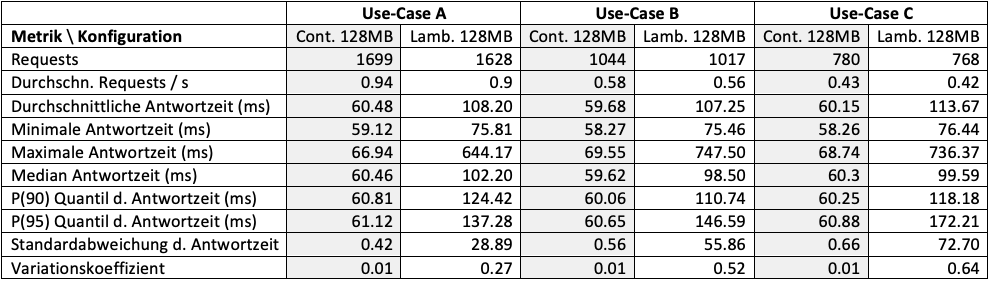
\includegraphics[width=\textwidth]{img/pipe128-comparison.png}
    \caption[Vergleich der Pipe-Clean Tests für 128MB]{Vergleich der Pipe-Clean Tests für 128MB}
    \label{fig:pipe128-comparison}
\end{figure}

Abbildung \ref{fig:pipe128-comparison} zeigt die Ergebnisse des Tests für die Funktionen mit 128MB CPU bzw. RAM. Es ist zu erkennen, dass die Container Anwendung in allen Fällen eine deutlich geringere Antwortzeit als die Lambda Anwendung aufweist. Im Median ist der Container bei Use-Case A etwa 41,74ms schneller als die Lambda-Funktion. Während die maximale Antwortzeit bei ersterer nur etwa 10,7\% über dem Median liegt, ist sie bei der Lambda-Funktion etwa 630\% über ihrem Median. Dass die Lambda-Anwendung eine überaus große Varianz in ihren Antwortzeiten aufweist, wird auch in ihrer Standardabweichung von bis zu 72ms deutlich, währende sie bei der Container Anwendung in allen drei Use-Cases unter 1ms liegt. Interessanterweise liegt die Antwortzeit der Lambda-Anwendung im Median in allen drei Use-Cases bei ähnlichen Werten um ca. 100ms. Andererseits nimmt die Standardabweichung und das P(95) Quantil der Antwortzeit bei Use-Case B im Vergleich zu Use-Case A deutlich zu. Und auch bei Use-Case C ist ein deutlicher Anstieg der Werte zu beobachten. Vermutlich ist dies auf die größere Anzahl an angefragten Endpunkten zurückzuführen, da dadurch mehr Coldstarts durchgeführt werden müssen. Auch bei der Container-Anwendung ist keine Veränderung der Median-Antwortzeit um ca. 60ms festzustellen. Die Standardabweichung der Antwortzeit erhöhte sich nur leicht von 0,42 auf 0,66.

\section{128MB Konfigurationen}
Zunächst werden alle Tests gegen die 128MB Konfigurationen ausgeführt. In den folgenden Sektionen wird dann die Speicher- und Prozessorgröße erhöht. 

\subsection{Stress-Tests}
Um RQ1 zu beantworten, muss zunächst die maximale Auslastung eines einzelnen Containers ermittelt werden. Dazu wurden mehrere Stress-Tests durchgeführt. Ein Stress-Test dient dazu, die Grenzen des SUTs herauszufinden. Da Lambda ein von Natur aus automatisch horizontal skalierendes System ist, werden die Test zunächst für die Container-Anwendung durchgeführt und im Anschluss die Lambda-Anwendung mit der gleichen Test-Konfiguration getestet. Dadurch kann das Verhalten der Funktionen bei langsamem Anstieg der Benutzer evaluiert werden. Die Anzahl der VUs wird bei den Stress-Tests wie von Molyneaux\cite{molyneaux_art_2014} empfohlen immer stufenweise erhöht. Das bedeutet, dass nach jedem Ramp-Up (ein linearer Anstieg) eine gleichlange Periode mit einer konstanten Anzahl an Benutzern folgt. Abbildung \ref{fig:stress-vus-example} verdeutlicht dies anhand eines Stress-Tests, bei dem bis zu 600 gleichzeitige Virtuelle Benutzer erstellt werden. In 60 Sekunden Zeitabschnitten werden nach und nach immer 60 Benutzer hinzugefügt. Daraufhin folgt eine weitere 60 Sekunden lange Periode, in der die Anzahl der VUs nicht weiter erhöht wird. Der gesamte Test hat demnach eine Dauer von 40 Minuten. Eine Cooldown-Phase nach den vollen 600 Benutzern wird hier nicht eingelegt, da das Skalierungsverhalten nicht untersucht wird.

\begin{figure}[H]
    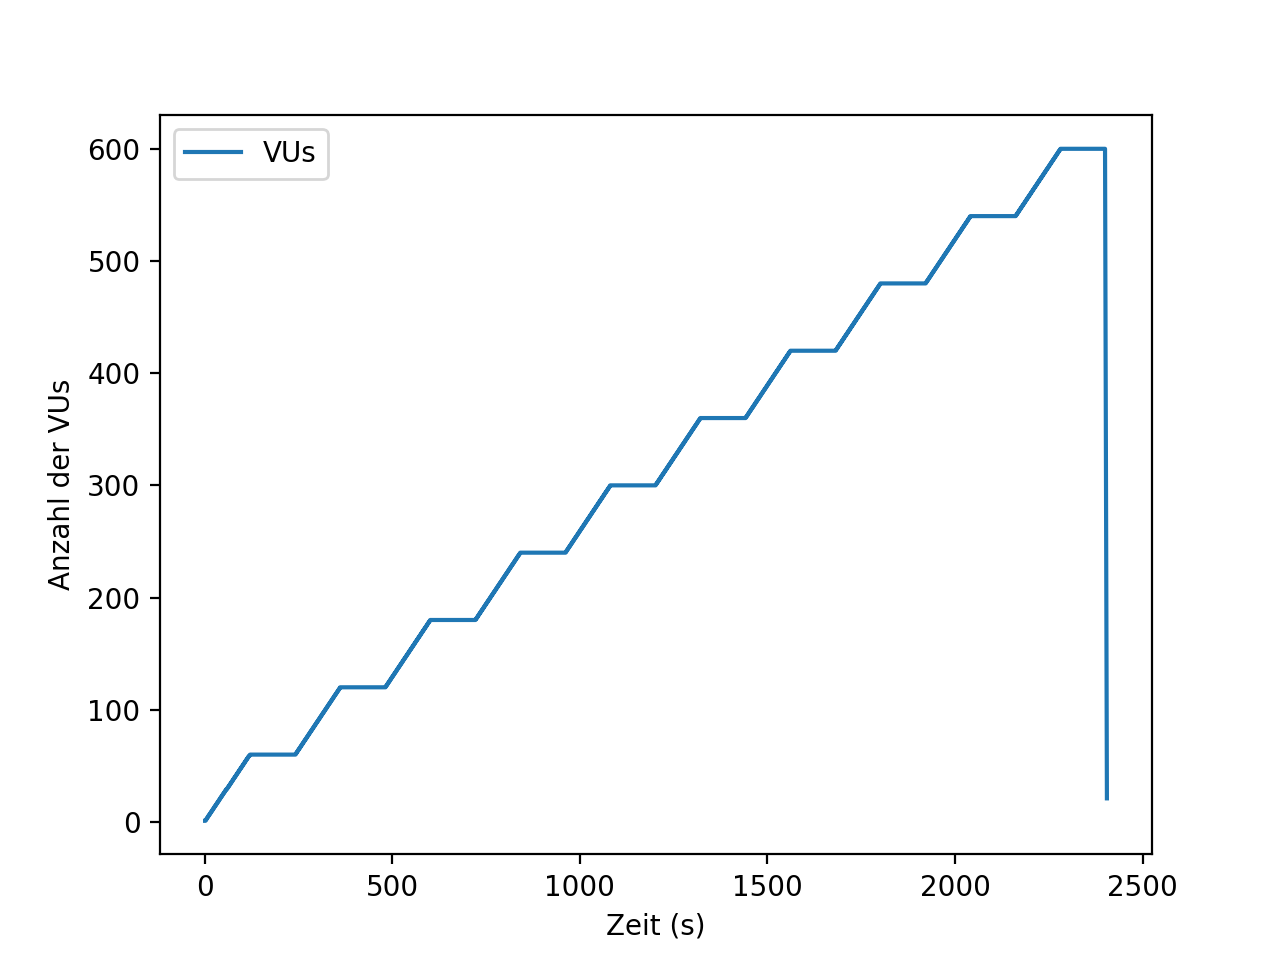
\includegraphics[width=\textwidth]{img/stress-vus-example.png}
    \caption[Beispiel-Anstieg der gleichzeitigen VUs für einen Stress Test]{Beispiel-Anstieg der gleichzeitigen VUs für einen Stress Test}
    \label{fig:stress-vus-example}
\end{figure}

\subsubsection{Container}
Für die containerisierte Anwendung in der 128MB Konfiguration wurden mehrere Stress-Tests durchgeführt, bis das Limit der gleichzeitigen Benutzer identifiziert werden konnte. Abbildung \ref{fig:fargate128-stress-comparison} zeigt die getesteten Use-Cases und die Stress-Test Konfiguration. 

\begin{figure}[H]
    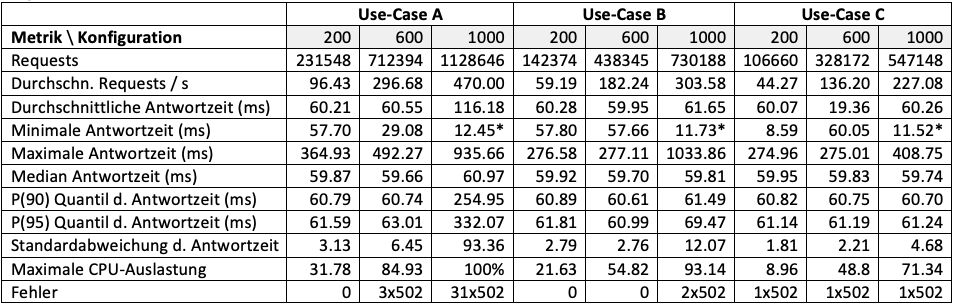
\includegraphics[width=\textwidth]{img/fargate128-stress-comparison.png}
    \caption[Fargate 128MB Stress-Test Vergleich]{Fargate 128MB Stress-Test Vergleich}
    \label{fig:fargate128-stress-comparison}
\end{figure}

Der erste Test wurde mit bis zu 200 Benutzern durchgeführt. Dabei konnte jedoch nur bis zu 32\% der CPU-Auslastung des Container-Clusters erreicht werden; In Use-Case B waren es sogar nur fast 22\%. Der geringen Auslastung entsprechend, war kaum eine Veränderung der Antwortzeiten gegenüber den Pipe-Clean Tests festzustellen (vgl. mit Abbildung \ref{fig:pipe128-comparison}). Einige Metriken lagen sogar unter den Grundwerten. Lediglich die maximale Antwortzeit hat sich bei allen Use-Cases, bspw. bei Use-Case A von 60,46ms auf 364,93ms, deutlich erhöht. Dies ist allerdings nur vereinzelt der Fall, da immer noch 95\% aller Anfragen innerhalb von ca. 62ms beantwortet werden und auch an der Standardabweichung hat sich nicht großartig verändert. 

Bei dem zweiten Stress-Test mit bis zu 600 VUs, änderte sich nicht viel im Vergleich zu dem Test mit 200 Benutzern. Es konnten zwar bis zu 84,93 Prozent CPU-Auslastung erreicht werden und die maximale Antwortzeit stieg erneut an, auf fast 500ms. Trotz dessen konnten von dem einzelnen Container 95\% der Anfragen innerhalb von knapp 63ms beantwortet werden. Problematisch zeigten sich hier drei Requests, die vom Server nicht mehr beantwortet werden konnten und den 502 Fehlercode zurücksendeten. Dies entspricht jedoch nur 0,00042\% aller in diesem Stress-Test durchgeführten Requests.

\begin{figure}[H]
    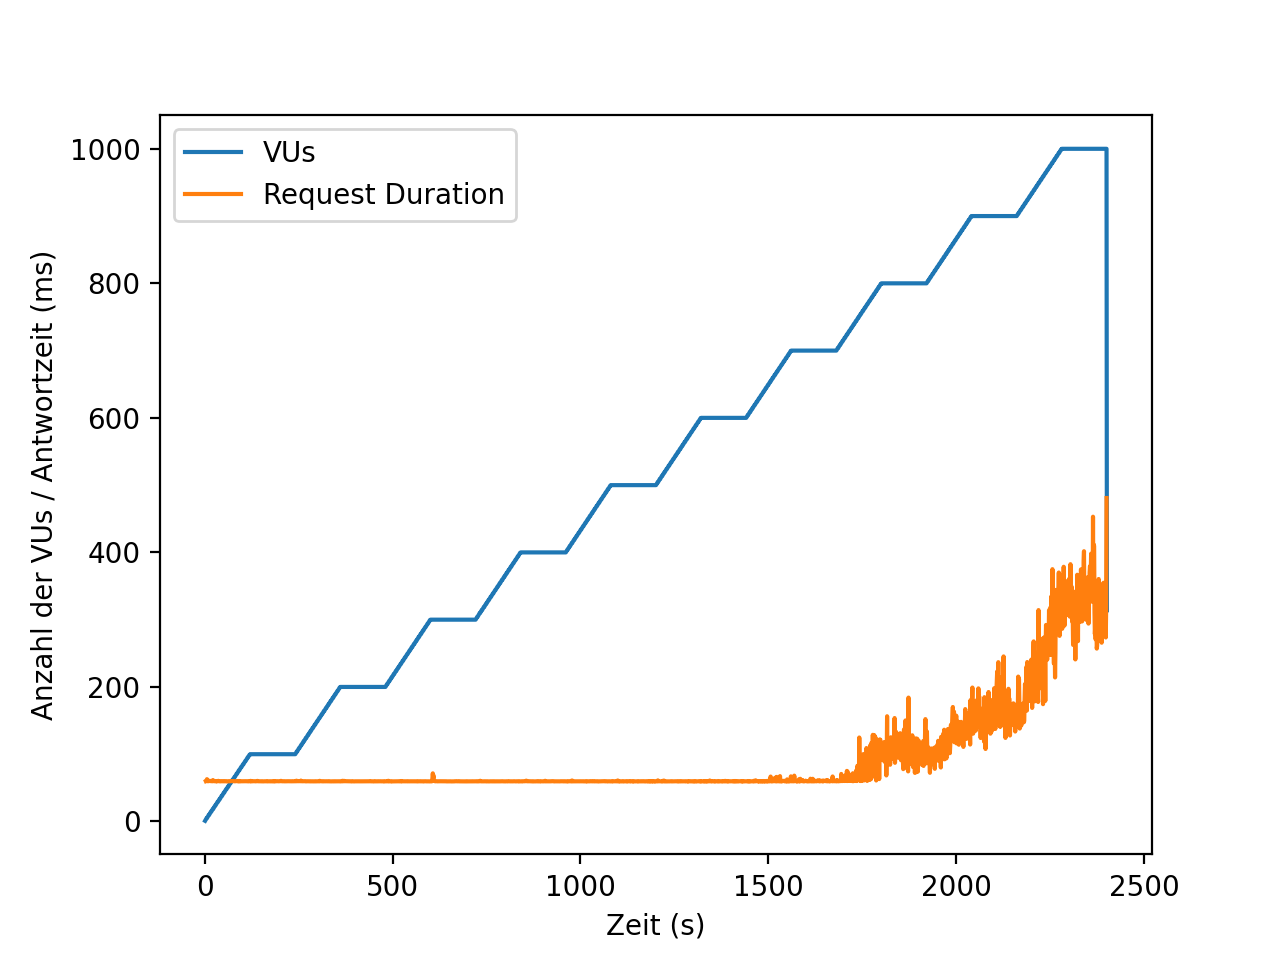
\includegraphics[width=\textwidth]{img/fargate128-stress1000.png}
    \caption[Container Stress-Test 1000VUs]{128MB Container Stress-Test 1000VUs Use-Case A}
    \label{fig:fargate128-stress1000}
\end{figure}

Der dritte Stress-Test für den 128MB Container wurde mit bis zu 1000 VUs durchgeführt. Abbildung \ref{fig:fargate128-stress1000} zeigt den zeitlichen Verlauf dieses Tests für Use-Case A. Es wird dabei die Anzahl der virtuellen Benutzer und die Antwortzeit im Median pro Sekunde dargestellt. Es wird deutlich, dass die Antwortzeit ab ca. 700 VUs deutlich ansteigt. Dies deckt sich der von AWS Cloudwatch gemessenen CPU-Auslastung von knapp unter 100\% die bei dieser Nutzerzahl gemessen wurde. In den Perioden mit konstanten Nutzerzahlen können die Requests besser verarbeitet werden und die Kurve geht wieder leicht herunter. Während des Tests wurden trotz einer CPU-Auslastung von teilweise 100\% nur 31 HTTP 502 Fehlercodes vom Server ausgelöst, was einer Quote von 0,0027\% entspricht. Die Antwortzeit konnte im Median weiterhin bei etwa 60ms gehalten werden; die durchschnittliche Antwortzeit stieg mit 116,8ms auf fast das doppelte des Grundwertes an.  
Bei Use-Case B lag die erreichte Prozessor-Auslastung bei 93,14\%. So wurden keine deutlichen Abweichungen ausgelöst. Die Standardabweichung stieg leicht an, liegt aber immer noch deutlich unter dem Wert des Pipe-Clean Tests der 128MB Lambda Funktion.

\subsubsection{Lambda}
Nachdem die maximale Performance des 128MB Containers ermittelt wurde, werden im Anschluss die gleichen Stress-Tests für die Lambda-Anwendung mit 128MB durchgeführt. Abbildung \ref{fig:lambda128-stress-comparison} zeigt die Ergebnisse. Für Use-Case A lässt sich erkennen, dass die Standardabweichung bei 200 und 600 VUs noch um die 19 beträgt, während bei 1000 Usern auf fast 55 ansteigt. Dies könnte allerdings an den extrem langen maximalen Antwortzeiten von bis zu 29.037ms liegen, die durch die Fehler verursacht werden. Die großen Fehler-Latenzen stehen im Gegensatz zu der Container Anwendung, bei der die maximale Antwortzeit immer noch knapp unter einer Sekunde lag. Auffallend ist, dass Fehler mit HTTP Statuscode 500 etwa 10s Antwortzeit aufweisen, während Fehler mit HTTP Statuscode 504 die fast 30s lange Latenz erzeugen. Die bei der Container-Anwendung erzeugten HTTP 502 Fehlercodes, führen stattdessen zu  Antwortzeiten von 12ms - 260ms. 

\begin{figure}[H]
    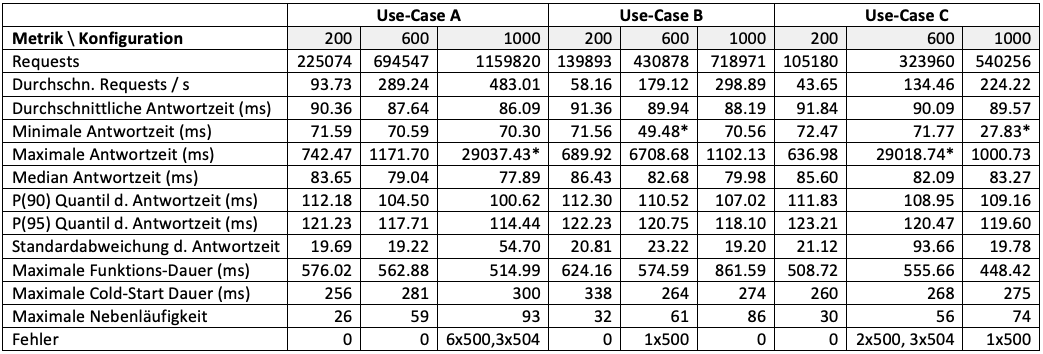
\includegraphics[width=\textwidth]{img/lambda128-stress-comparison.png}
    \caption[Lambda 128MB Stress-Test Vergleich]{Lambda 128MB Stress-Test Vergleich}
    \label{fig:lambda128-stress-comparison}
\end{figure}

Bei der Durchführung der Stress-Tests für die 128MB Lambda-Anwendung fällt außerdem auf, dass die Antwortzeit im Median bei steigenden Nutzerzahlen zu sinken scheint. Bei bis zu 200 VUs lag sie für Use-Case A noch bei 83.65ms, während sie bei bis zu 1000 VUs auf 77.89ms sank. Die Werte für Use-Case B scheinen einem ähnlichen Prinzip zu unterliegen. Es ist jedoch aktuell nicht bekannt, warum dies der Fall ist. Vermutlich provisioniert AWS die Funktionen schneller je mehr Anfragen sie erhalten. Trotz dessen, liegt die Antwortzeit im Median immer noch deutlich über der des 128MB Containers; die Differenz ist allerdings im Vergleich zu den Pipe-Clean Tests von 41,74ms auf 16.92ms gesunken (Use-Case A).

Zwischen den Use-Cases wird ebenfalls ein Unterschied in der Anzahl der nebenläufigen (concurrent) Lambda-Funktionen deutlich. Während bei 200 und 600 VUs für Use-Case B noch mehr Funktionen bereitgestellt wurden als für Use-Case A, zeigt sich für 1000 VUs ein umgekehrtes Bild. In diesem Fall, übertrifft der erste Use-Case den zweiten um 7 nebenläufige Funktionen. Dies ist interessant gegenüber RQ5, da es der Hypothese widerspricht, dass bei einer einzelnen angefragten Funktion weniger Coldstarts durchgeführt werden müssen als bei mehreren Funktionen (H5). Grund dafür ist vermutlich jedoch die geringere Anzahl der Requests pro Sekunde bei Use-Case B. 

\subsection{Spike-Test}
Für RQ2 soll die Performance unter schnell ansteigenden Nutzerzahlen ermittelt werde. Dazu wird ein Spike-Test durchgeführt. Ziel dessen ist es, die Performance der Anwendungen unter rasch ansteigender Last zu ermitteln. In den bisherigen Stress-Tests wurden nur langsame Anstiege (Ramp-Ups) durchgeführt. Nun soll nach einer kurzen Initialisierungsphase mit normalem Load (200VUs) eine schneller Anstieg auf 600 Virtuelle Benutzer erfolgen. Diese Benutzeranzahl wurde gewählt, um den Container nicht zu überlasten.

\subsubsection{Container}


\subsubsection{Lambda}